%%%%%%%%%%%%%%%%%%%%%%%%%%%%%%%%%%%%%%%%%%%%%%%%%%%%%%%%%%%%
%%

%%%%%%%%%%%%%%%%%%%%%%%%%%%%%%%%%%%%%%%%%%%%%%%%%%%%%%%%%%%%%
%% FSBI presentation on spatial stats and mixed fisheries %%%
%%%%%%%%%%%%%%%%%%%%%%%%%%%%%%%%%%%%%%%%%%%%%%%%%%%%%%%%%%%%%

\documentclass[xcolor=x11names,compress]{beamer}

%% General document %%%%%%%%%%%%%%%%%%%%%%%%%%%%%%%%%%
\usepackage[english]{babel}
\usepackage{graphicx}
\usepackage{epstopdf}
\usepackage{subcaption}
\captionsetup{compatibility=false}
\usepackage{tikz}
\usepackage[utf8]{inputenc}
\usepackage{times}
\usepackage[T1]{fontenc}
\usetikzlibrary{decorations.fractals}
%%%%%%%%%%%%%%%%%%%%%%%%%%%%%%%%%%%%%%%%%%%%%%%%%%%%%%

%% Beamer Layout %%%%%%%%%%%%%%%%%%%%%%%%%%%%%%%%%%
\useoutertheme[subsection=false,shadow]{miniframes}
\useinnertheme{default}
\usefonttheme{serif}
\usepackage{palatino}

\setbeamerfont{title like}{shape=\scshape}
\setbeamerfont{frametitle}{shape=\scshape}

\setbeamercolor*{lower separation line head}{bg=DeepSkyBlue4} 
\setbeamercolor*{normal text}{fg=black,bg=white} 
\setbeamercolor*{alerted text}{fg=red} 
\setbeamercolor*{example text}{fg=black} 
\setbeamercolor*{structure}{fg=black} 
 
\setbeamercolor*{palette tertiary}{fg=black,bg=black!10} 
\setbeamercolor*{palette quaternary}{fg=black,bg=black!10} 

\definecolor{mygreen}{cmyk}{0.82,0.11,1,0.25}
\setbeamertemplate{blocks}[rounded][shadow=false]
\addtobeamertemplate{block begin}{\pgfsetfillopacity{0.8}}{\pgfsetfillopacity{1}}
\setbeamercolor{structure}{fg=mygreen}

\renewcommand{\(}{\begin{columns}}
\renewcommand{\)}{\end{columns}}
\newcommand{\<}[1]{\begin{column}{#1}}
\renewcommand{\>}{\end{column}}
\graphicspath{{figures/}}

%%%%%%%%%
%%%%%%%%%%%%%%%%%%%%%%%%%%%%%%%%%%%%%%%%%%%%%%%%%%
 
\titlegraphic{
	\includegraphics[width = 1.5cm]{MRFC_Bubble} \hspace*{4.6cm}
	\includegraphics[width = 2.5cm]{seedcorn_logo_white_navy_bkgd}  \\
	\includegraphics[width = 2.5cm]{gmit-logo} \hspace*{1cm}
	\includegraphics[width = 2.5cm]{MARES} \hspace{1cm}
	\includegraphics[width = 2.5cm]{cefas_fish_white_dark_blue_bkgd}
	}

%%\AtBeginSection{\frame{\sectionpage}}



%%%%%%%%%%%%%%%%%%%%%%%%%%%%%%%%%%%%%%%%%%%%%%%%%%%%%%%%%
									      
\begin{document}

\addtocounter{framenumber}{-1}

%%%%%%%%%%%%%%%%%%%%%%%%%%%%%%%%%%%%%%%%%%%%%%%%%%%%%%
%%%%%%%%%%%%%%%%%%%%%%%%%%%%%%%%%%%%%%%%%%%%%%%%%%%%%%
\begin{frame}
\title{Using spatio-temporal population models to inform mixed-fishery management}

\author{Paul Dolder}
\author[shortname]{Paul J. Dolder, \inst{1,2} \and 
	James Thorson \inst{3} \and 
	Cóilín Minto\inst{1}}
\vspace{-0.5cm}

\institute[shortinst]{\inst{1}Galway-Mayo Institute of Technology, Ireland
	\and \vspace{-0.2cm}
\inst{2} Centre for Environment, Fisheries and Aquaculture Science, UK \and
\vspace{-0.2cm}
\inst{3} North West Fisheries Science Center, NOAA, USA}

\date{6 July 2017 \\ FSBI Symposium, Exeter, UK}
\titlepage
\end{frame}

%%%%%%%%%%%%%%%%%%%%%%%%%%%%%%%%%%%%%%%%%%%%%%%%%%%%%%%%%%%%%%
%%%%%%%%%%%%%%%%%%%%%%%%%%%%%%%%%%%%%%%%%%%%%%%%%%%%%%%%%%%%%%

%%%%%%%%%%%%%%%%%%%%%%%%%%%%%%%%%%%%%%%%%%%%%%%%%%%%%%
%%%%%%%%%%%%%%%%%%%%%%%%%%%%%%%%%%%%%%%%%%%%%%%%%%%%%%

\section{Background}
\subsection{Blah}
\begin{frame}{Scene setting}

\begin{columns}
	
	
\column{0.3\paperwidth}
\vspace{-1.5cm}
\includegraphics[height=3cm, width=4cm]{techInteractions}\\ 
\includegraphics[height=3cm, width=4cm]{discarding} 

\column{0.7\paperwidth}

\begin{itemize}
	\small	
	\setlength\itemsep{1em}
	\pause
	\item Mixed fisheries, where more than one species are caught together,
		are the main type of marine fishery worldwide. \pause
	\item In the EU where fisheries are managed by single 'stock' quotas,
		mixed fisheries have led to the overexploitation of weaker
		stocks, where fishing continues for healthier fisheries. \pause
	\item As the EU moves towards a 'landings obligation' - all fish will
		caught count against quota. \pause
	\item Fish populations are heterogeneously distributed in space and
		time. Increased interest is spatio-temporal dynamics to see how
		spatial measures can contribute to sustainable fisheries. 
\end{itemize}
	
\end{columns}

\end{frame}

\begin{frame}{Motivation}

\begin{columns}
\column{0.4\paperwidth}
\includegraphics[width  = \linewidth]{Irish_catch_comp}
\\
\tiny
\hspace{0.2cm}
\textit{Gerritsen et al 129-130 (2012). Fisheries Research} 
\column{0.6\paperwidth}
\includegraphics[width  = \linewidth]{All_species_finescale}

\end{columns}
\end{frame}

\begin{frame}{Motivation}

\begin{columns}
	
\column{0.3\paperwidth}
\includegraphics[width  = \linewidth]{boat}

\column{0.7\paperwidth}
\begin{itemize}
\small	
\setlength\itemsep{1em}

	\item We wanted to understand how space can be used to separate catches
		of different stocks in highly mixed fisheries. \pause
	\item There are difficulties in combining different sources of data in
		fisheries modelling: collected for different purposes,
		different temporal and spatial coverage. \pause
	\item Needed a coherent framework: looked to developments in
		geostatistical methods, particularly applied to the types of
		data we have. \pause
	\item Provide insight into how far spatial measures and avoidance can
		go to improving sustainability of mixed fisheries.

\end{itemize}



\end{columns}

\end{frame}

%%%%%%%%%%%%%%%%%%%%%%%%%%%%%%%%%%%%%%%%%%%%%%%%%%%%%%
%%%%%%%%%%%%%%%%%%%%%%%%%%%%%%%%%%%%%%%%%%%%%%%%%%%%%%

\section{Methods}
\subsection{Blah}

\begin{frame}

Modelling framework (VAST):

\begin{columns}

	\column{0.2\paperwidth}
	
	\includegraphics[width  = 0.8\linewidth]{survey_locations}

	\column{0.8\paperwidth}
\pause

\begin{enumerate}
	\small
	\setlength\itemsep{1em}

	\item Joint Dynamic Species Distribution Model (JDSDM) able to take
		account of latent (unobserved) drivers which affect species
		distribution and density for one or more species, \pause
	\item the use of Gaussian Markov Random Fields (GMRFs) to model the
		variation in probability of occurrence and density as a
		three-dimensional multivariate process (latitude, longitude and
		time) \pause
	\item separate modelling of encounter probability and positive catch
		rates (so called 'delta' and 'hurdle' models),  \pause
	\item set in a mixed modelling framework allowing the incorporation of
		both systematic (fixed) effects and random effects. 
	
\end{enumerate}

\end{columns}

\end{frame}


%\begin{frame}{Factor analysis}

%	Simple explanation - use simple figures / diagrams
	
%	Reduces complexity of the problem - explain trends as a combination of
%factors (latent variables)

%Can provide insight to the community dynamics

	
%\end{frame}

%\begin{frame}{Gaussian Random Fields}

%	Tobler's law - "Everything is related to everything else, but near
%	things are more related than distant things (Tobler, 1970).

%	Such relationships can provide information for poorly sampled species
%	through inference of their relationships

%	Again, include simple diagrammatic example - take people through it!


%\end{frame}

%\begin{frame}{delta-GLMM and covariates}

%Surveys often are not coordinated, inconsistent design - need to take account
%of these differences.

%Can take account of both fixed effects (e.g. gear) and random effects in a
%mixed modelling framework.

	
%\end{frame}

%%%%%%%%%%%%%%%%%%%%%%%%%%%%%%%%%%%%%%%%%%%%%%%%%%%%%%%%%%%%%
%%%%%%%%%%%%%%%%%%%%%%%%%%%%%%%%%%%%%%%%%%%%%%%%%%%%%%%%%%%%%

\section{Data}
\subsection{Blah}

\begin{frame}{}
\centering
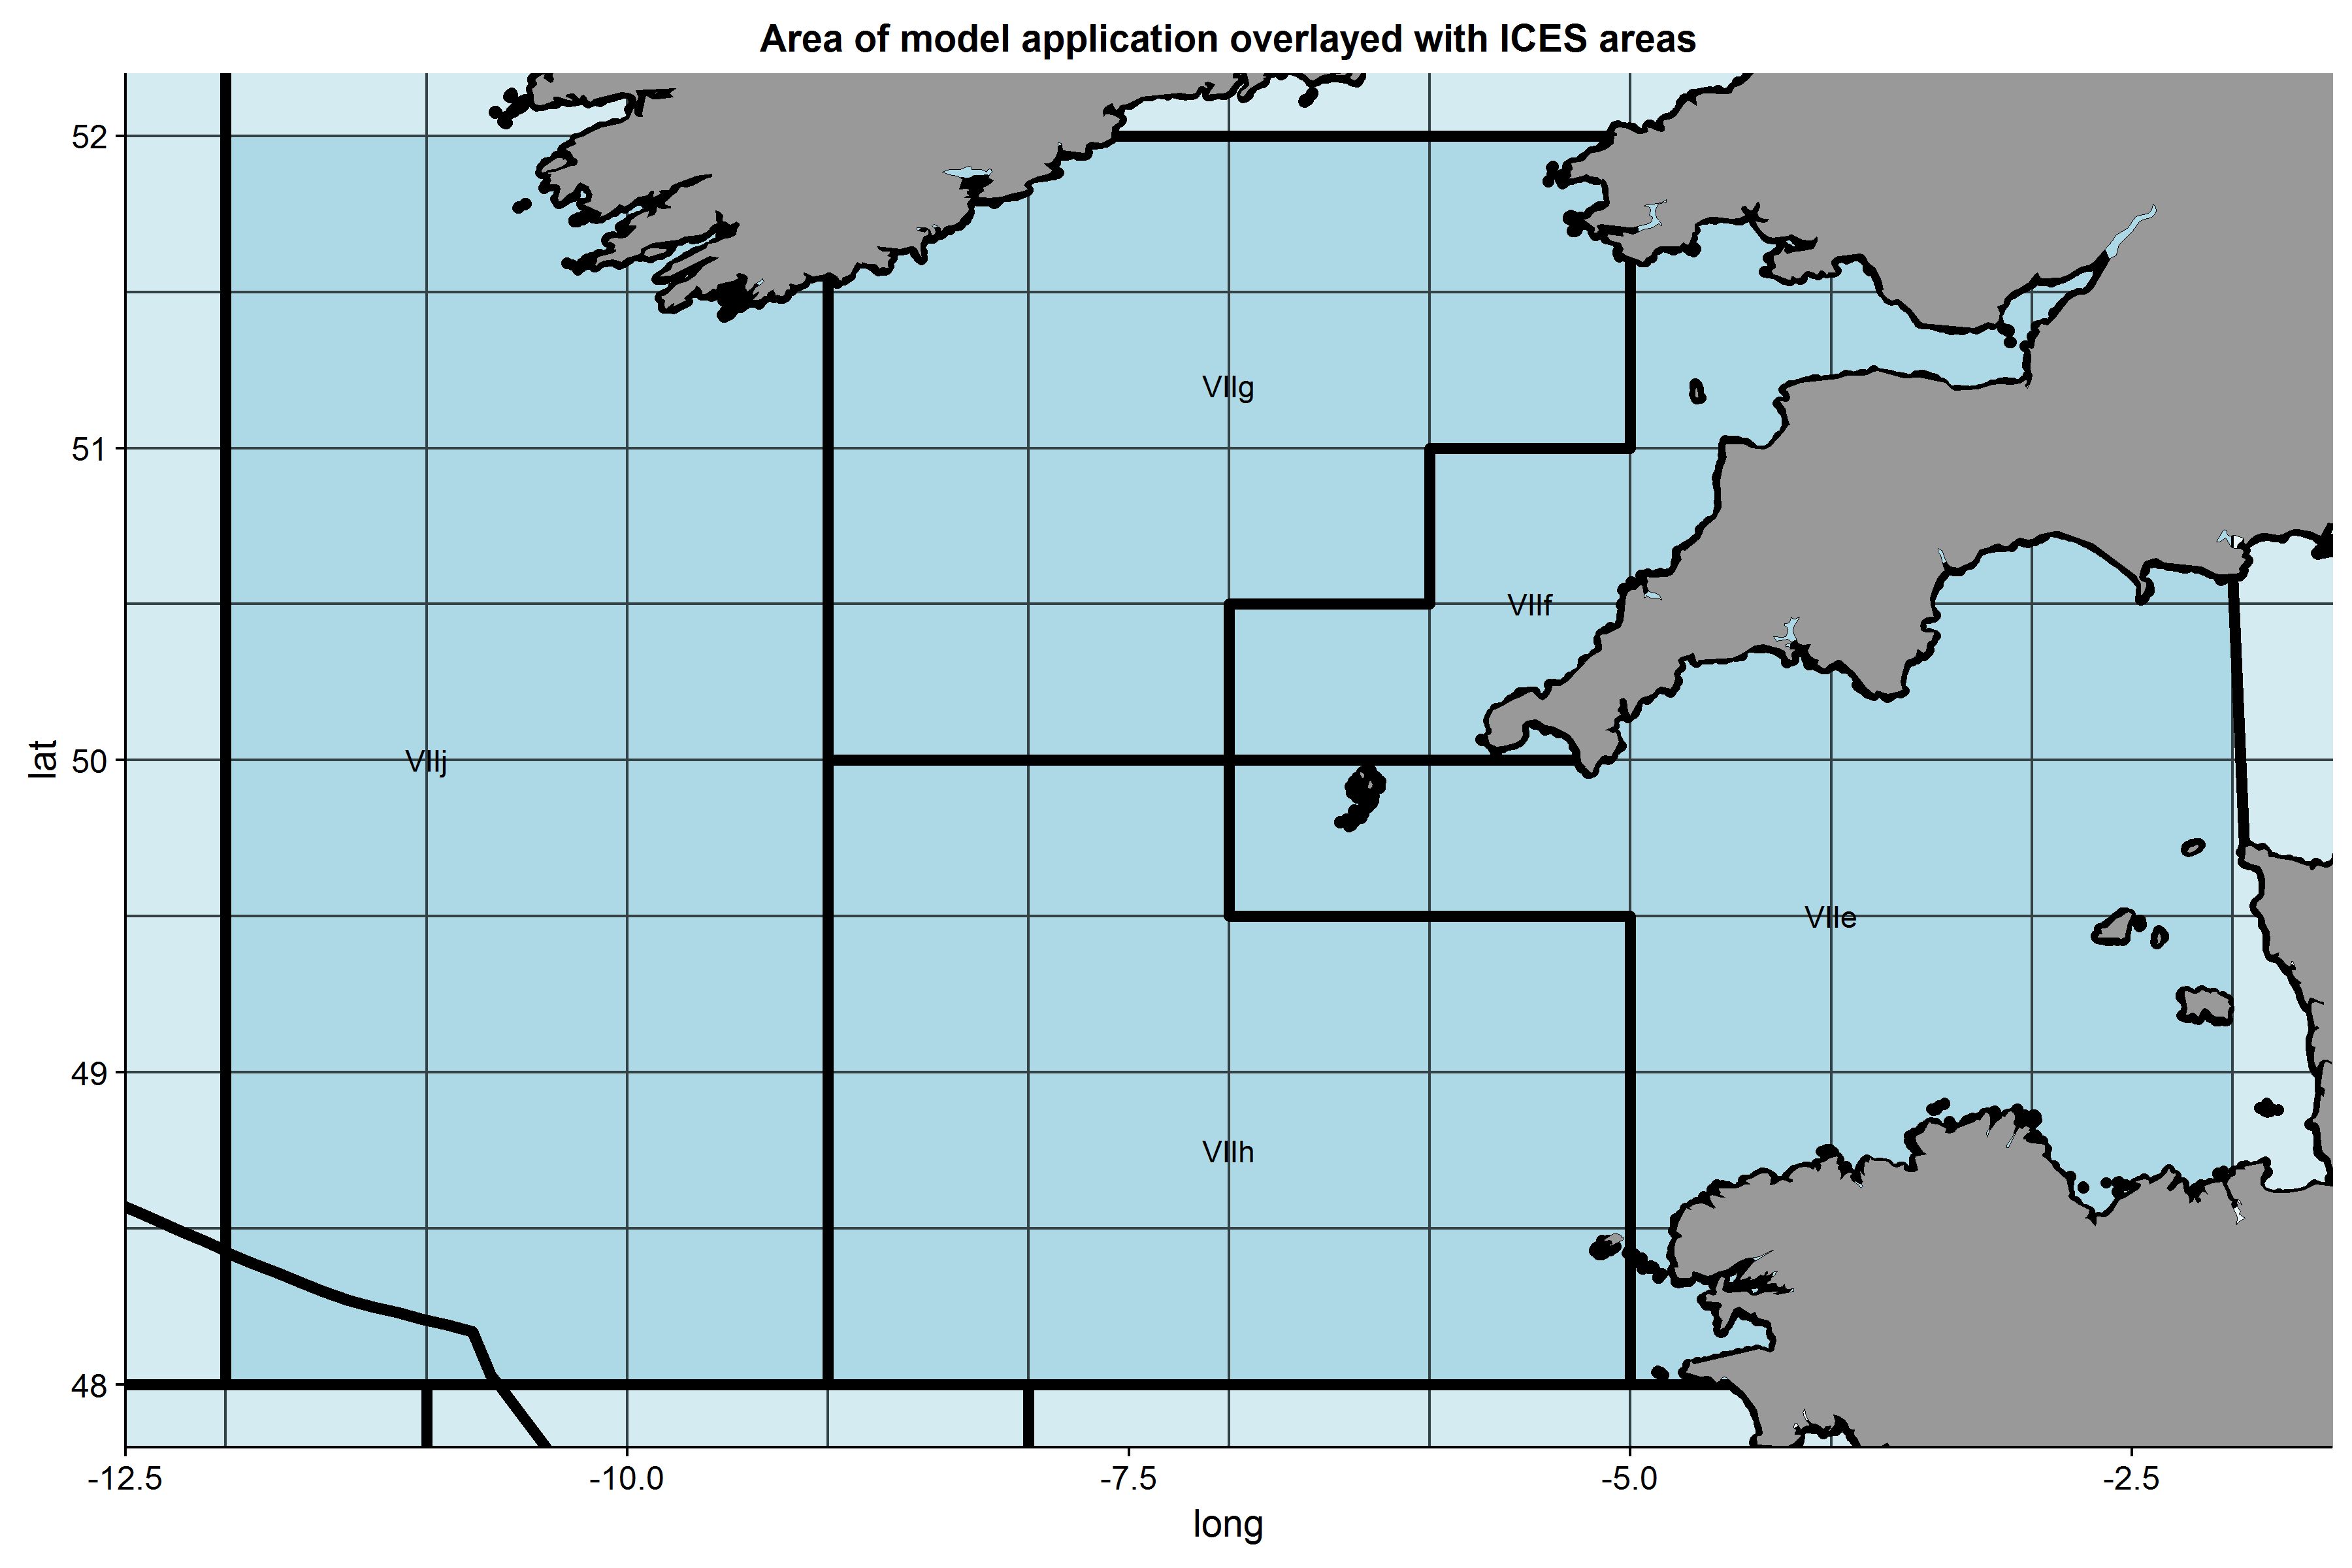
\includegraphics[width=\linewidth]{AreaMap}

\end{frame}

\begin{frame}

\begin{table}[!htb]
	\tiny
	\center
	\begin{tabular}{ p{1.5cm} p{3cm} p{2cm} p{1.5cm} }
		\hline
		Survey code    & Name 	& Gear & Temporal extent \\
		\hline
		CEXP / IE-IGFS & Celtic Explorer (IE)   & Otter trawl & 2003 - 2015 \\
		CARLHELMAR     & Carlhelmar (UK)	& Commercial beam trawl & 1989 - 2013 \\
		NWGFS          & North West groundfish survey (UK) & Beam trawl & 1988 - 2015 \\
		Q1SWBEAM       & Quarter 1 south-west beam trawl survey (UK) 	& beam trawl & 2006 - 2015 \\
		Q4SWIBTS       & Quarter 4 south-west international bottom trawl survey (UK) & Otter trawl & 2003 - 2010 \\
		THA2 / EVHOE    & EVHOE survey on Thalasa (FR) & Otter trawl & 1997 - 2015 \\
		WCGFS          & Wstern channel groundfish survey (UK) & Otter
		trawl (Portuguese high headline) & 1982 - 2004 \\
		\hline
	\end{tabular}
	
\end{table}

\includegraphics[width=0.6\linewidth]{Survey_effort_by_year-1}
\includegraphics[width=0.4\linewidth]{cefas_endeavour}

\end{frame}

\begin{frame}
	\centering
	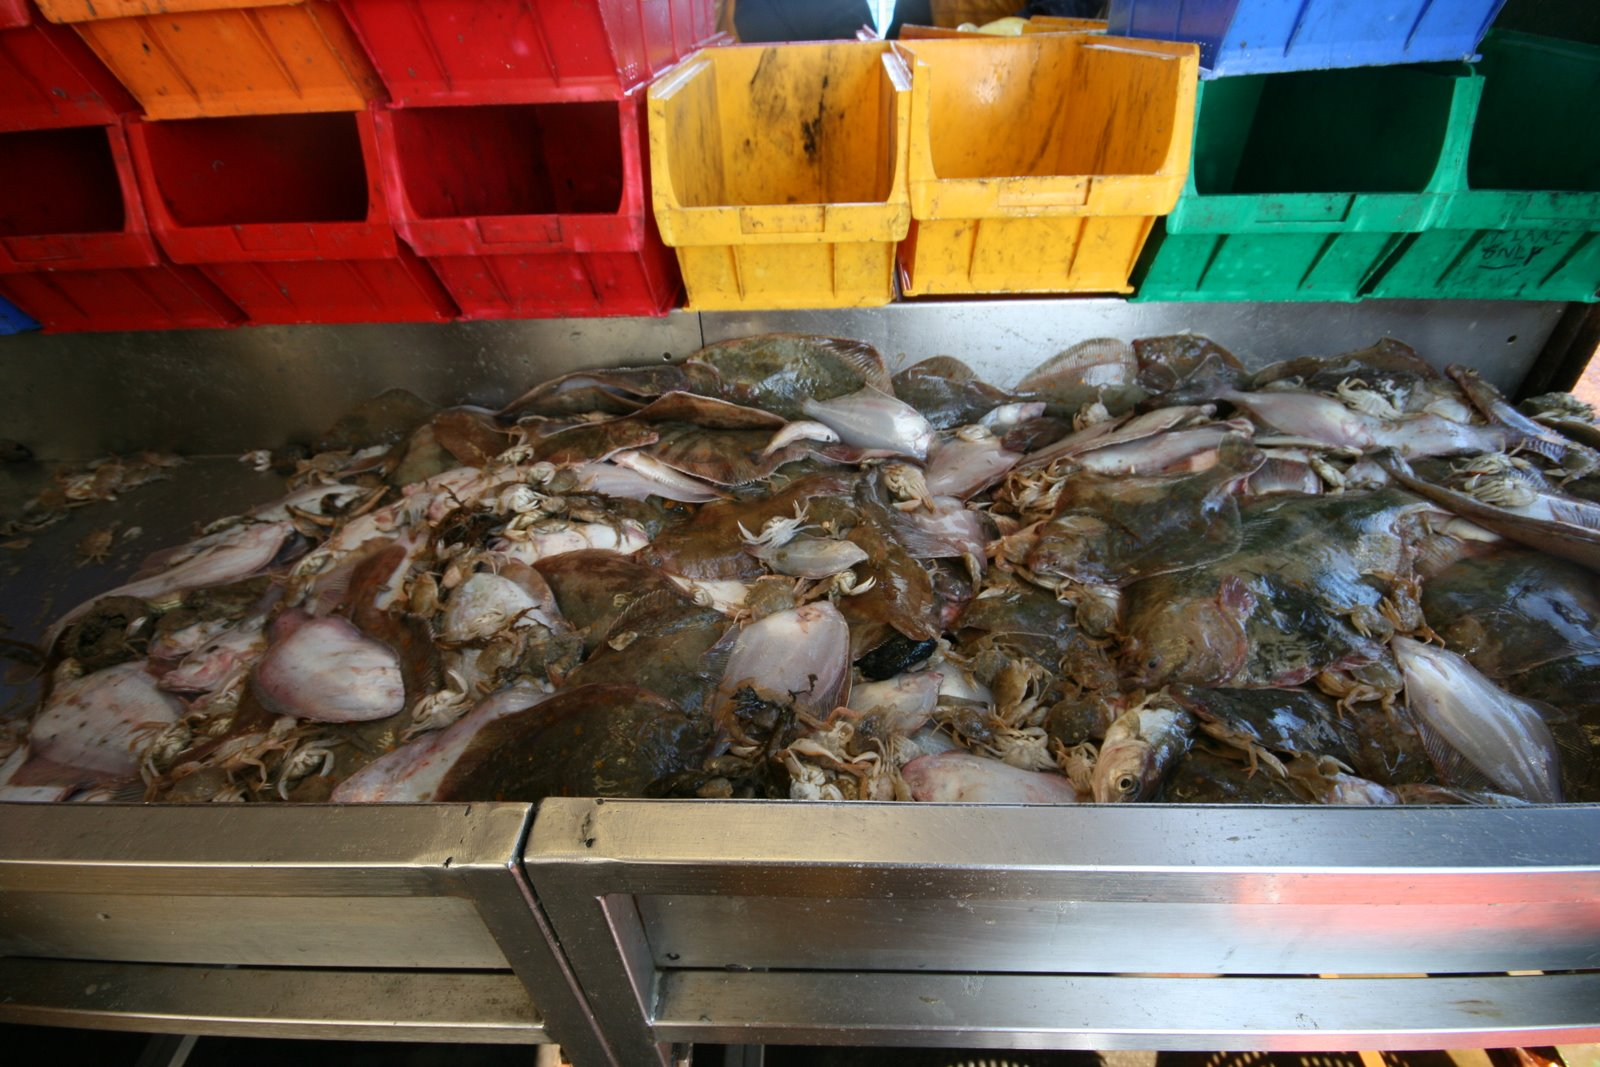
\includegraphics[height = 3cm]{IMG_9160}
	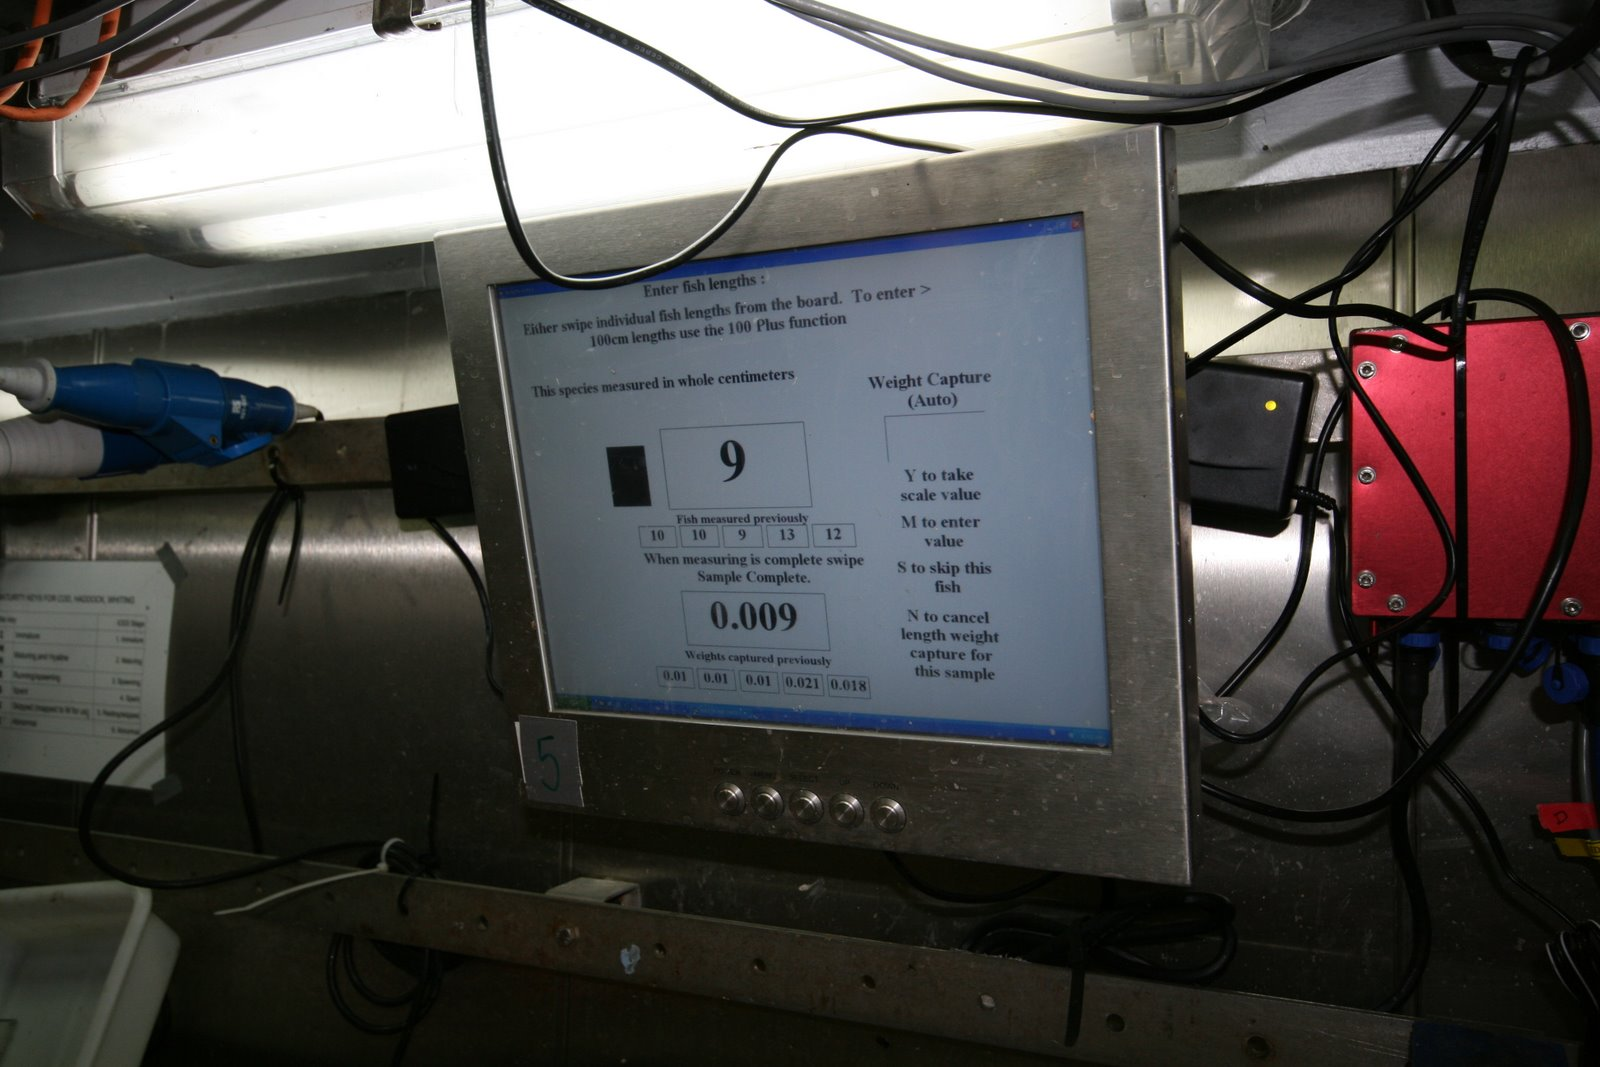
\includegraphics[height = 3cm]{IMG_9267} \\
	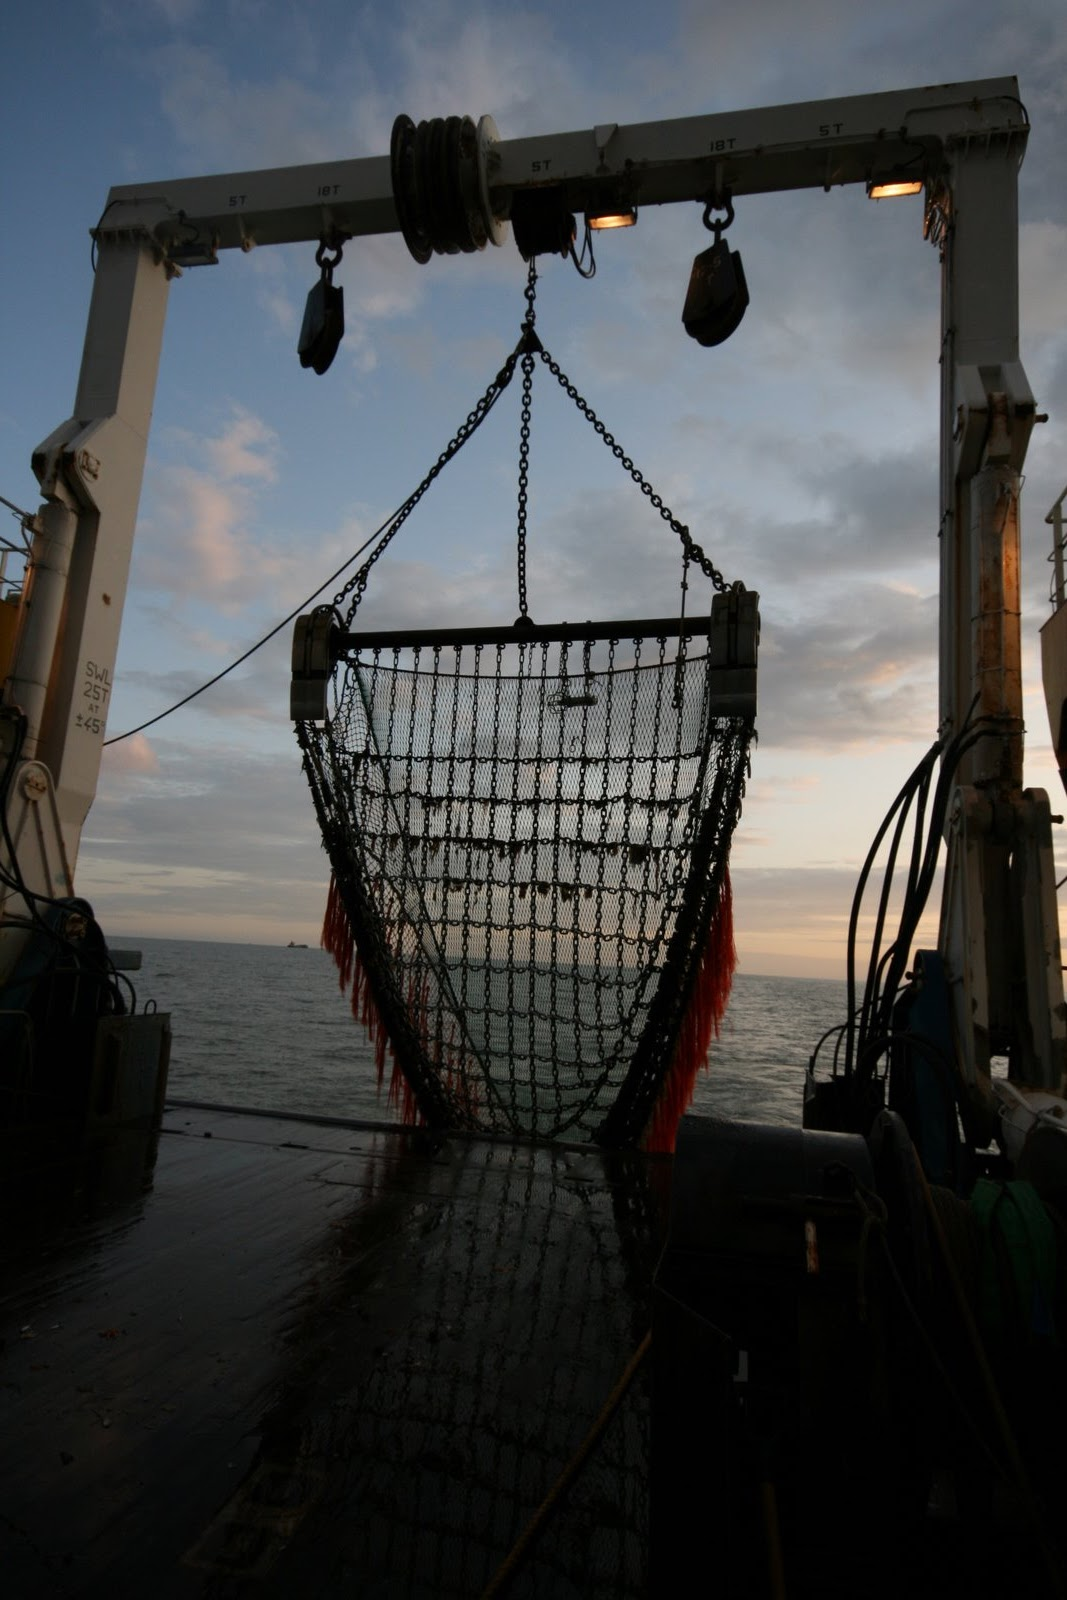
\includegraphics[height = 4cm]{IMG_9192}
	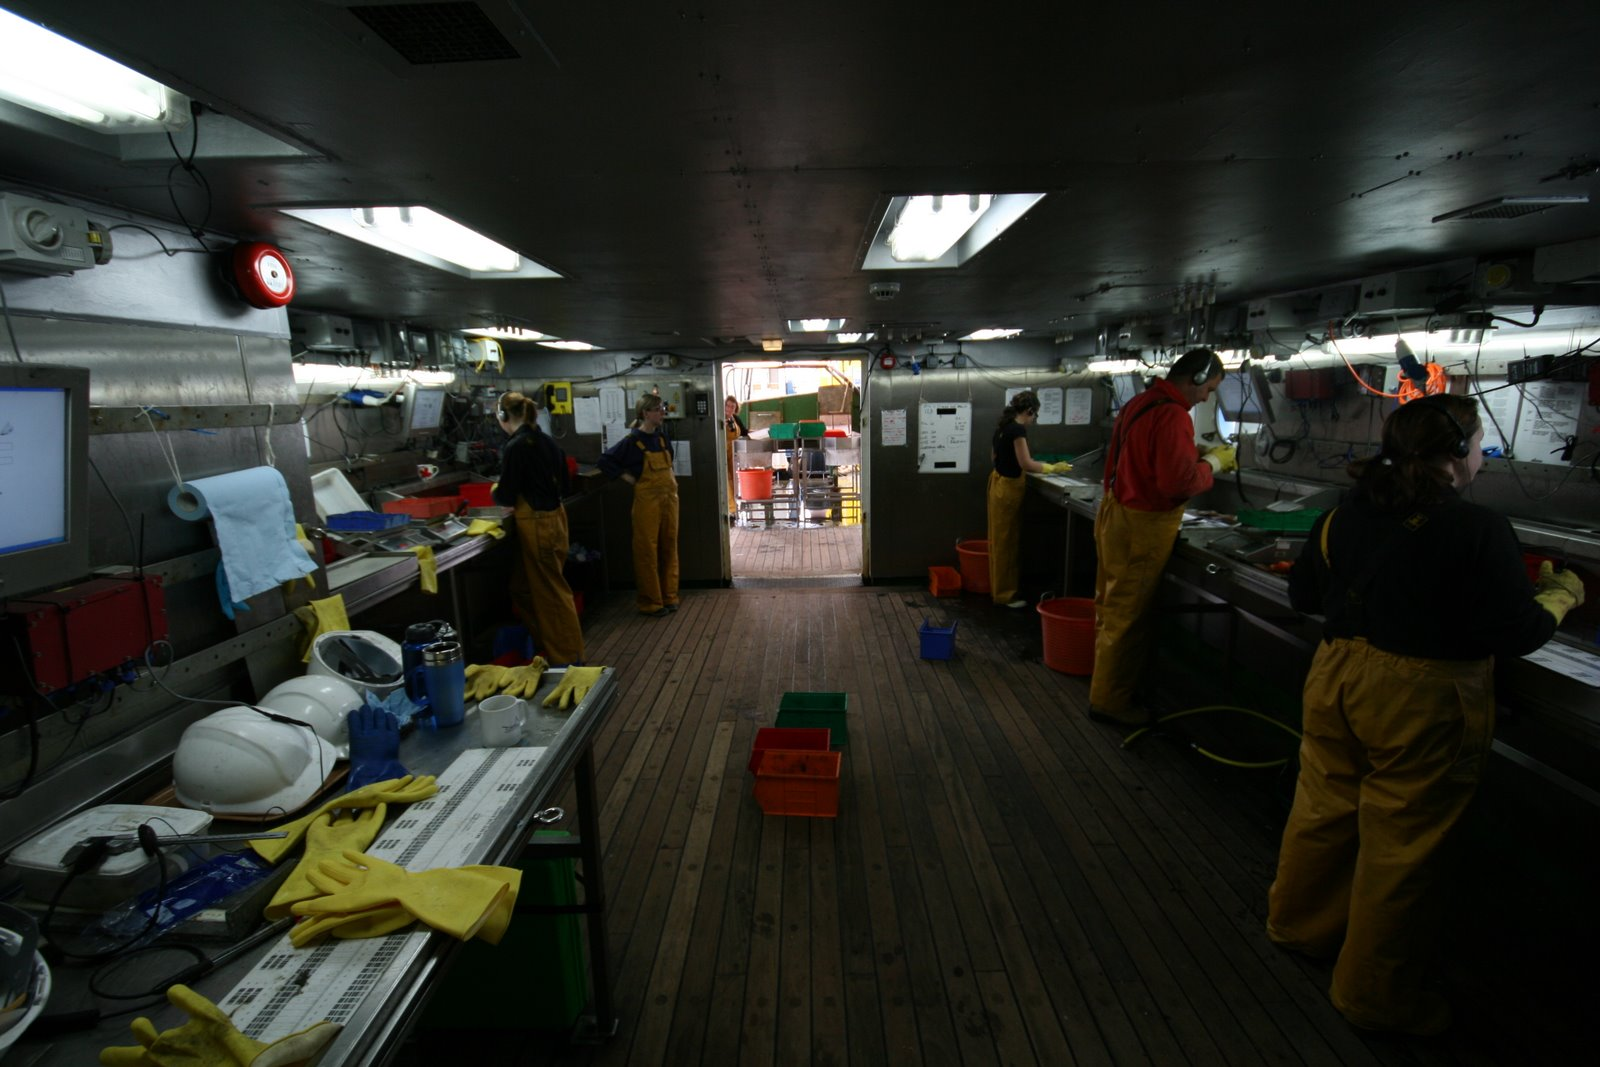
\includegraphics[height = 4cm]{IMG_9279}
	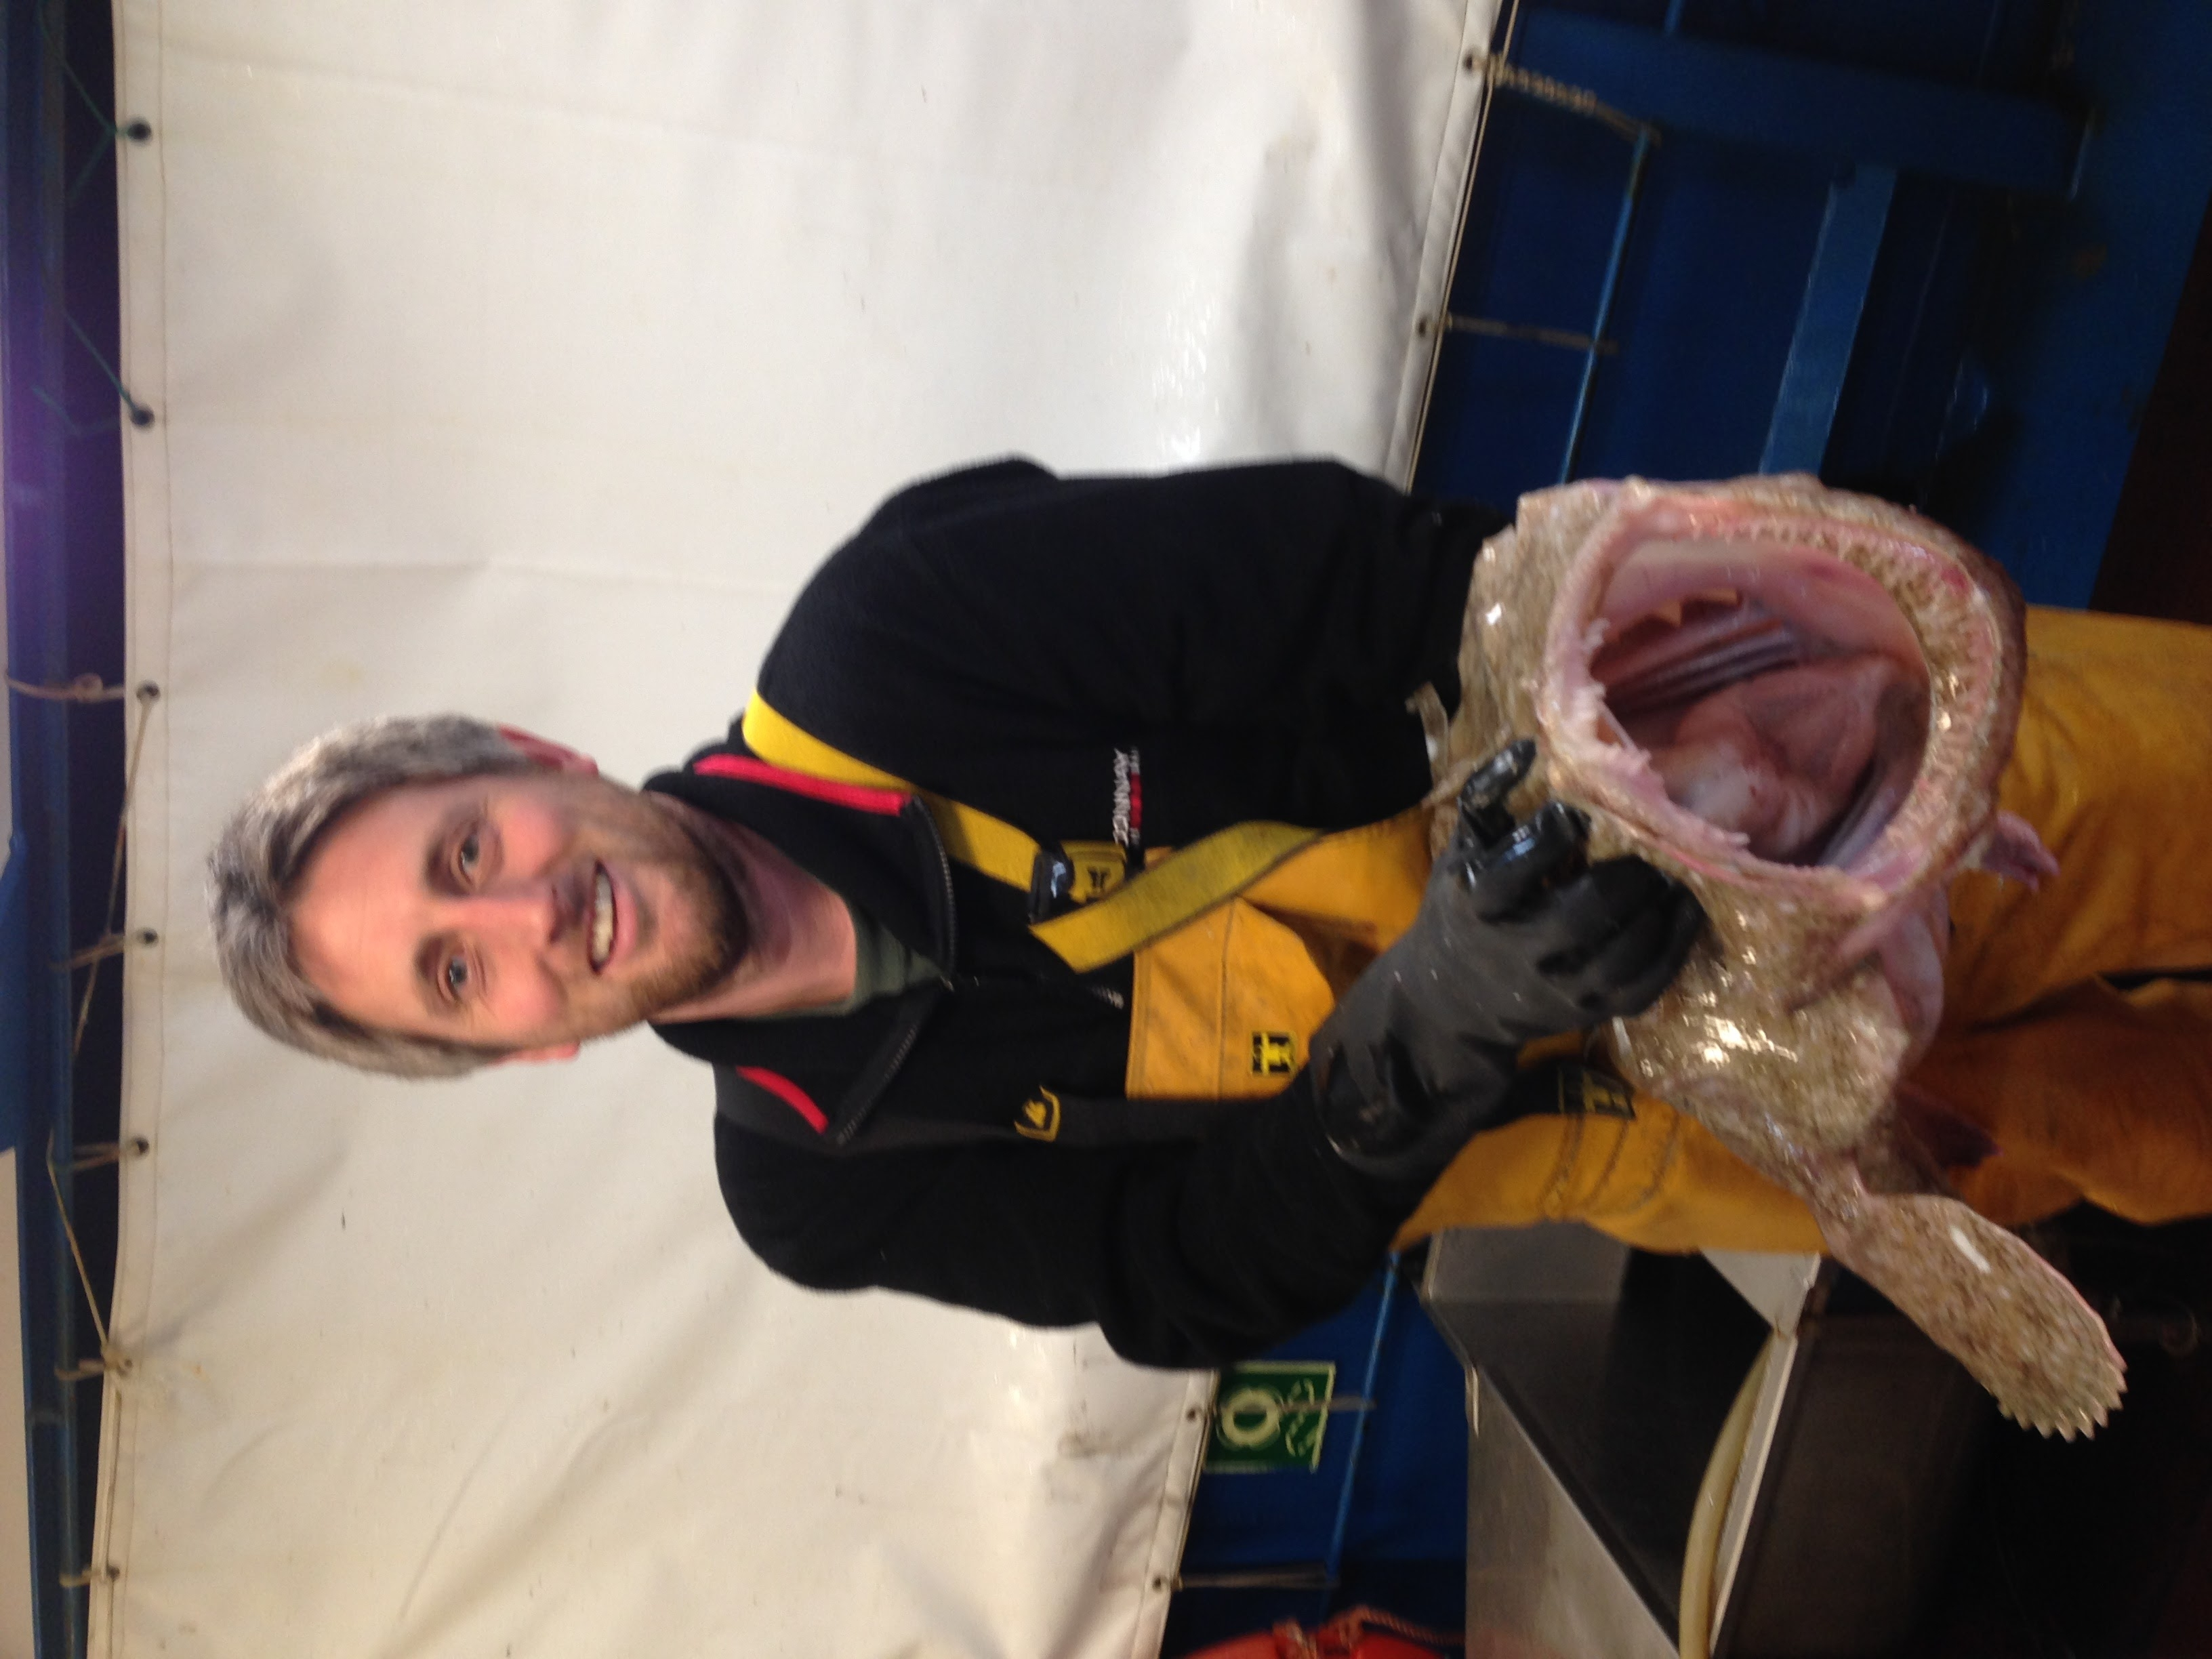
\includegraphics[height = 4cm]{Paul_Dolder}
\end{frame}

\begin{frame}

\begin{columns}
\column{0.3\linewidth}
\includegraphics[width = \linewidth]{"Legend"}

\column{0.8\linewidth}
\begin{table}[!htb]
	\tiny
	\center
	\begin{tabular}{ p{1cm} p{2cm} p{3cm} p{1cm}}
		\hline
		Species code & Common name              & Species & MCRS (cm) \\
		\hline
		juv          & Juvenile                 & & \\
		adu          & Adult                    & & \\
		\hline
		bud          & Black bellied anglerfish & \textit{Lophius budgessa} & 32* \\
		cod          & Atlantic cod             & \textit{Gadus morhua} & 35 \\
		had          & Atlatic haddock          & \textit{Melanogrammus	aeglefinus} & 30 \\
		hke          & Atlantic hake            & \textit{Merluccius merluccius} & 27 \\
		meg          & Megrim                   & \textit{Lepidorhombus whiffiagonis} & 20\\
		pisc         & White bellied anglerfish & \textit{Lophius piscatorius} & 32* \\
		ple          & European Plaice          & \textit{Pleuronectes platessa} & 27 \\
		sol          & Common sole              & \textit{Solea solea} & 24 \\
		whg          & Atlantic whiting         & \textit{Merlangius merlangus} & 27 \\
		\hline
		\end{tabular}
		*Monkfish species estimated based on a 500g minimum marketing weight


\end{table}

\end{columns}
\end{frame}

\begin{frame}{Spatial fields}
\centering
\includegraphics[width=0.9\paperwidth]{SpatialDataAndKnotsLand} \\
\vspace{-0.5cm}
\includegraphics[width=0.2\paperwidth]{inlamesh}

\end{frame}


\begin{frame}
\centering
\includegraphics[width = \linewidth]{"time"}

\end{frame}

\section{Some findings}
\subsection{Blah}

%%% cod - adult and juvenile 
\begin{frame}
\begin{tikzpicture}
	\centering
  \node (img1) at (1,1) {\includegraphics[height=8cm]{"Field_Dens--Gadus morhua_Adu"}};
       \pause
  \node (img3) at (1,1) {\includegraphics[height=8cm]{"Field_Dens--Gadus morhua_Juv"}};
\end{tikzpicture}
\end{frame}


\begin{frame}
	What about the fish as a community; what common spatial trends do we observe?
\end{frame}


\begin{frame}{Spatial patterns driving distributions and density}

\centering
\tiny
Spatial Encounter Probability
\includegraphics[width = \linewidth]{"Figure 2 - SpatialFactorLoadingsOmega1"}
\\
Spatial Density
\includegraphics[width = \linewidth]{"Figure 2 - SpatialFactorLoadingsOmega2"}
	
\end{frame}

\begin{frame}{What drives these patterns?}
\centering
\pause
\includegraphics[width = 0.4\linewidth]{"Factor1_DepthO1"}
\includegraphics[width = 0.5\linewidth]{"Depth"} \\
\pause
\includegraphics[width = 0.4\linewidth]{"Factor1_HabitatO1"}
\includegraphics[width = 0.5\linewidth]{"Substrate"}
\tiny
\hspace{2cm} Data: EUSeapMap; EMODnet bathymetry portal. \\
\pause
\tiny
\textcolor{red}{First factor shows strong correlation with depth for encounter probability
(-0.85, -0.88 to -0.81) and density (-0.71, -0.77 to -0.65). 80 \% of variance
explained by depth and habitat: 9/10 of that by depth.}

\end{frame}

\begin{frame}
        How stable are the spatial patterns over time ?	
\end{frame}

\begin{frame}{Temporal changes in common trends}
\centering
\includegraphics[width = 0.8\linewidth]{"Suppl - SpatioTempLoadingsEpsilon1Pres"}
\end{frame}

\begin{frame}{}
\centering
\includegraphics[width = 0.6\linewidth]{"Temp"} \\
\pause
\includegraphics[width = 0.6\linewidth]{"Factor1_Temp"} \\
\tiny
Data: NOAA High Resolution SST data. 
\end{frame}

\begin{frame}
Are the same factors driving all or some of the species distributions, when
taking account of the yearly variation?
\end{frame}

%%% PCA type plots - encounter
\begin{frame}
\begin{tikzpicture}
  \node (img1) at (1,1) {\includegraphics[height=7cm]{"Figure 3 - PCAstyle_Plots_SpatioTempEncBase"}};
     \node (img2) at (7,1) {\includegraphics[height=7cm]{"Legend"}};
       \pause
	  \node (img3) at (1,1) {\includegraphics[height=7cm]{"Figure 3 - PCAstyle_Plots_SpatioTempEnc1"}};
	  \pause
	  \node (img4) at (1,1) {\includegraphics[height = 7cm]{"Figure 3 - PCAstyle_Plots_SpatioTempEnc2"}};
	  \pause
	  \node (img5) at (1,1) {\includegraphics[height = 7cm]{"Figure 3 - PCAstyle_Plots_SpatioTempEnc3"}};
	  \pause
	  \node (img6) at (1,1) {\includegraphics[height = 7cm]{"Figure 3 - PCAstyle_Plots_SpatioTempEnc"}};
	  \end{tikzpicture}
\end{frame}

%%% PCA type plots - density 
\begin{frame}
\begin{tikzpicture}
  \node (img1) at (1,1) {\includegraphics[height=7cm]{"Figure 3 - PCAstyle_Plots_SpatioTempDenBase"}};
     \node (img2) at (7,1) {\includegraphics[height=7cm]{"Legend"}};
       \pause
	  \node (img3) at (1,1) {\includegraphics[height=7cm]{"Figure 3 - PCAstyle_Plots_SpatioTempDen1"}};
	  \pause
	  \node (img4) at (1,1) {\includegraphics[height = 7cm]{"Figure 3 - PCAstyle_Plots_SpatioTempDen2"}};
	  \pause
	  \node (img5) at (1,1) {\includegraphics[height = 7cm]{"Figure 3 - PCAstyle_Plots_SpatioTempDen3"}};
	  \pause
	  \node (img6) at (1,1) {\includegraphics[height = 7cm]{"Figure 3 - PCAstyle_Plots_SpatioTempDen"}};
	  \end{tikzpicture}
\end{frame}

%%% Correlations

\begin{frame}{}
\begin{tikzpicture}
  \node (img1) at (1,1) {\includegraphics[height=7cm]{"Figure 1 - Omega1_Correlations_norect"}};
  \node (img2) at (7,1) {\includegraphics[height=7cm]{"Legend"}};
       \pause
	\node (img1) at (1,1) {\includegraphics[height=7cm]{"Figure 1 -	Omega1_Correlations_blank"}};
\end{tikzpicture}
\end{frame}

\begin{frame}{}
\begin{tikzpicture}
  \node (img1) at (1,1) {\includegraphics[height=7cm]{"Figure 1 - Omega2_Correlations_norect"}};
  \node (img2) at (7,1) {\includegraphics[height=7cm]{"Legend"}};
       \pause
	\node (img1) at (1,1) {\includegraphics[height=7cm]{"Figure 1 -	Omega2_Correlations_blank"}};
\end{tikzpicture}
\end{frame}


%%%%%%%%%%%%%%%%%%%%%%%%%%%%%%%%%%%%%%%%%%%%%%%%%%%%%%%%%%
%%%%%%%%%%%%%%%%%%%%%%%%%%%%%%%%%%%%%%%%%%%%%%%%%%%%%%%%%%
\section{Implications for mixed fishery mgmt}
\subsection{Blah}

\begin{frame}{So what does this mean for mixed fisheries management ?}

	\begin{itemize}
		\item Method for reducing dimensionality of the 'mixed fishery
			problem': identifies the associations among species;
		\item Clear separation among 3 groups of species indicating
			that spatial avoidance is possible;
		\item More challenging within a group where strong association
			in both distribution and density exists;
		\item However,...
	\end{itemize}

\end{frame}

\begin{frame}{Species density overlaps}
	
\centering
\includegraphics[width = \linewidth]{"Figure 4 - DensityDifferencesFigureswithCC"}

\end{frame}


\section{Conclusions}
\subsection{Blah}

\begin{frame}{Key messages}
\begin{itemize}
\small	
\setlength\itemsep{1em}
	\item Method for identifying common trends in distribution and density
		of species at a scale consistent with the data, robust and
		takes account of covariance structure;
	\item Applied to main Celtic Sea commercial fish species indicates
		spatial separation among three broad species groups: demersal
		roundfish, flatfish and deeper water species;
	\item Factor analysis shows the dynamics are driven common spatial
		trends - indicates the strong associations among species groups
		are driven by the environment; 
	\item Implications for spatial avoidance under the EU landings
		obligation: how far can space be used to match catch to
		available quota?
\end{itemize}

\end{frame}


\begin{frame}{Acknowledgements}
\centering
\includegraphics[height=3cm]{"Coilin_Minto"} \hspace{1cm}
\includegraphics[height=3cm]{"Jim_Thorson"} \\
\vspace{1cm}
\includegraphics[width = 2.5cm]{seedcorn_logo_white_navy_bkgd} 
\hspace{0.5cm}
\includegraphics[width = 2.5cm]{MARES}  
\hspace{0.5cm}
\includegraphics[width = 2.5cm]{ichec_logo} 
\hspace{0.5cm}
\includegraphics[width = 2.5cm]{FSBI} 

\tiny 
References: \url{www.github.com/james-thorson/VAST}

\end{frame}


\begin{frame}{} 

\begin{tikzpicture}
\node (img1) {\includegraphics[width = 10cm]{/home/paul/Dropbox/MARES_PhD/jointprod_study/docs/paper_headers/Selection_012}};
\pause
\node (img2) at (img1.south) {\includegraphics[width = 10cm]{/home/paul/Dropbox/MARES_PhD/jointprod_study/docs/paper_headers/Selection_013}};
\pause
\node (img3) at (img2.north) {\includegraphics[width = 10cm]{/home/paul/Dropbox/MARES_PhD/jointprod_study/docs/paper_headers/Selection_011}};
\pause
\node (img4) at (img3.south) {\includegraphics[width = 10cm]{/home/paul/Dropbox/MARES_PhD/jointprod_study/docs/paper_headers/Selection_014}};
\pause
\node (img5) at (img4.north) {\includegraphics[width = 10cm]{/home/paul/Dropbox/MARES_PhD/jointprod_study/docs/paper_headers/Selection_010}};

\end{tikzpicture}

\end{frame}


%%%%%%%%%%%%%%%%%%%%%%%%%%%%%%%%%%%%%%%%%%%%%%%%%%%%%%
%%%%%%% Back up slides: equations etc...

\appendix
\section{Add. slides}
\subsection{Blahi}


\begin{frame}{Spatial coverage}

\centering
\includegraphics[width=1\linewidth]{Survey_locations-1}

\end{frame}


\begin{frame}{Methodology summary}

\begin{itemize}
	\small
	\setlength\itemsep{2em}

	\item Mesh construction: A spatial grid is constructed based on optimal
		clustering of the available point data using a k-means
		algorithm to provide \textit{n} knots representing the gaussian
		random fields used to derive spatial encounter probability and
		density estimates.

	\item  Associations among species / species-groups are modelled through
		implementing a factor analysis decomposition to define a
		function for each factor that returns a positive or negative
		association of one or more species with any location. Thus
		log-density of any species can then be described as a linear
		combination of factors:
		\begin{equation}
			\theta_{p}(s,t) = \sum_{j=1}^{n_{j}}
			L_{p,j}\psi_{j}(s,t) +\sum_{k=1}^{n_{k}}
			\gamma_{k,p}\chi_{k}(s,t)
		\end{equation}
	
\end{itemize}

\end{frame}

\begin{frame}{Methodology summary}
	\begin{itemize}
	\setlength\itemsep{2em}
	\small

	\item Spatio-temporal encounter probability and positive catch rates
		are modelled separately with spatio-temporal encounter
		probability modelled using a logit-link linear predictor;
		\begin{equation}
			logit[p(s_{i},p_{i},t_{i})] = \gamma_{p}(p_{i},t_{i}) +
			\varepsilon_{p}(s_{i},p_{i},t_{i}) + \delta_{p}(p_{i},
			v_{i})
		\end{equation}

		and positive catch rates modelling using a gamma- distribution
		\begin{equation}
			gamma[r(s_{i},p_{i},t_{i})] = \gamma_{p}(p_{i},t_{i}) +
			\varepsilon_{p}(s_{i},p_{i},t_{i}) + \delta_{p}(p_{i},
			v_{i})
		\end{equation}

\end{itemize}

\end{frame}

\begin{frame}{Methodology summary}
	\begin{itemize}
	\setlength\itemsep{2em}
	\small

	\item The spatio-temporal variation is modelled using a Gaussian
		Markov Random Field (GMRF) where catch data in nearby locations
		can be correlated, allowing inference about poorly sampled
		locations. 
	\item Specify a probability distribution for spatio-temporal
		variation in both encounter probability and positive catch rate, 
		$\varepsilon_{*}(s,p,t)$, with a three-dimensional multivariate 
		normal distribution so that:
		\begin{equation}
			vec[\mathbf{E}_{*}(t)] \sim MVN(0,\mathbf{R}_{*} \otimes
			\mathbf{V}_{{\varepsilon}{*}})
		\end{equation}
	\end{itemize}
	\centering
	\includegraphics[width=0.5\linewidth]{Matern}

\end{frame}

\begin{frame}{Methodology summary}
	\begin{itemize}
	\setlength\itemsep{2em}
	\small

	\item Vessels as either fixed or random effect, as well as predictive
		covariates (e.g. habitat quality, depth, temperature etc..) 
	\item Parameter estimation through Laplace approximation of the
		marginal likelihood using Template Model Builder (TMB).

	\item The index of abundance for species $p$ can then be derived from
		the summation of the spatio-temporal density estimates. 
		
		\begin{equation} I(p,t) =
			\sum_{s=1}^{n_{s}} a(s) \cdot
			logit^{-1}[\gamma_{p}(p,t) + \varepsilon_{p}(s,p,t)]
			\cdot exp[\gamma_{r}(p,t) + \varepsilon_{r}(s,p,t)]
		\end{equation}
\end{itemize}

\end{frame}

\begin{frame}{Setup}

\begin{itemize}
	\setlength\itemsep{2em}
	\small
	\item The data was constrained to 1990 - 2015, reflecting the period
		during which the most spatially consistent data were available.
	\item The GMRF was set to 250 knots based on a compromise between
		spatial disaggregation and computational efficiency.
	\item The number of factors for the factor analysis decomposition set
		at nine (which explained \textgreater 95 \% of the variance in
		the encounter probability and density).
\end{itemize}

\begin{table}[!htb]
	\tiny
	\center
	\begin{tabular}{ p{1cm} p{2cm} p{2cm} p{1cm} p{1cm} }
		\hline
		Model & Catchability covariates & Density covariates & No Fixed
		effects & No Random effects \\
		\hline
		M0 & Vessel as Random effect & None  & 1462 & 129276 \\
		M1 & Vessel*Species group as fixed effect & None & 1674 & 129276   \\
		M2 & Vessel*Species group as fixed effect & Habitat and depth
		as fixed covariates & 1688 & 129276 \\ 
		\hline
	\end{tabular}
\end{table}

\end{frame}

\begin{frame}
\centering
\includegraphics[width=0.5\paperwidth]{"Suppl - QEstimatesALL"}

\end{frame}

\begin{frame}{Q-Q plots}
\centering
\includegraphics[width=0.47\linewidth]{Diag--Encounter_prob}
\includegraphics[width=0.5\linewidth]{Q-Q_plot}

\end{frame}

\begin{frame}{Spatial correlation}
	\centering
\includegraphics[width=0.5\linewidth]{Aniso}
\end{frame}


%%%%%%%%%%%%%%%%%%%%%%%%%%%%%%%%%%%%%%%%%%%%%%%%%%%%%%
\end{document}
%%%%%%%%%%%%%%%%%%%%%%%%%%%%%%%%%%%%%%%%%%%%%%%%%%%%%%
%%%%%%%%%%%%%%%%%%%%%%%%%%%%%%%%%%%%%%%%%%%%%%%%%%%%%%
